%%%%%%%%%%%%%%%%%%%%%%%%%%%%%%%
%%%%%%%%%%%%%%%%%%%%%%%%%%%%%%%
%%%%%%%%%%%%%%%%%%%%%%%%%%%%%%%
% !TEX root = main.tex

\section{Introduction}

It has recently become possible to train much larger artificial neural networks than ever before. 

\editbox{write some intro fluff here vvvv}

Recent progress, enabled by Convnets \cite{LeCun89}

these new large networks are breaking previous performance records handily. Also unsupervised work: \cite{Le-2011-ICA} trained large unsupervised network using...

Most of these use combinations of learned convolutional features, pooling over fixed local regions, and normalization of responses based on the responses of other units in the same layer (a basic form of inhibition or local competition, which has a similar effect to ``explaining away'')

(speculation) It is interesting to think that, while we previously fought in a regime where mostly we tried to push performance, and most small performance gains well understood -- that is, the field of machine learning was largely a art of synthesizing functions that worked better and better -- we may soon be entering an era of the field where we have things that are so large and work so well that the performance will outpace our understanding. This will push the  field into a decidedly different regime, one of almost observational science where we merely poke things that work magically well to slowly remove their mystique.

Grand speculation aside, here we seek to understand a few properties of one of the larger class of convolutional neural networks trained using supervised backprop.

((examples))
((diff datasets))
((but same features!))

(((( two Gabor features from very different networks ))))

\editbox{write some intro fluff here ----}

Many trained networks reported recently in the literature --- unsupervised and supervised alike --- exhibit a curious aspect in common: they all learn features that resemble Gabor filters in the first layer (see Figure~\ref{fig:layer1}) \todo{fix broken figure ref here}. The appearance of these Gabor filters is so common that to obtain anything else on a natural-image dataset causes suspicion of poorly chosen hyperparameters or a software bug. 
%In fact, this paper's authors are now used to checking for Gabor features in the first layer simply to assure ourselves that the training is at least partially working.

Because finding Gabor features on the first layer seems to occur regardless of the exact cost function and natural image dataset used, we may call these these features \emph{general}. On the other hand, we know that the last layer of a trained network will depend greatly on the chosen \{network model, dataset\} combination. For example, for networks trained toward a supervised classification objective, each output unit will be specific to a particular class, at least to the extent that training is successful. In this sense, let's say that the last layer features are \emph{specific}. So far these terms are only intuitively defined, but we shall provide a candidate for a more rigorous definition below. \todo{Consider something like: ``Empirically, we know that these filter are generic because they can be transferred to other networks and perform well [cites]. Transferring information learned on one task or dataset to a new task or data set is know as \emph{Transfer Learning} [cites].''}

If these Gabor features of the first features are general, and the features of the last layer are specific, there must be a transition from general to specific somewhere in the network. This observation raises a few questions:

\begin{itemize}
	\item Can we quantify the degree to which a particular layer is general or specific?
	\item For a particular deep network, does the transition occur suddenly from layer $n$ to $n+1$, or is it spread out over several layers?
	\item Where does this transition take place: near the bottom, middle, or top of the network?
\end{itemize}

Once one has general features from some layer of a base network trained on a dataset, a common trick is to repurpose the features, or \emph{transfer} them, to another task. The process that is usually followed is to create a new network containing as its first $n$ layers the first $n$ layers of the base network, with the rest of the layers in the new network randomly initialized and trained toward the second task. When following this path, one can choose to backpropagate the errors from the new task into the base features to \emph{fine-tune} them to the new task, or they can be left frozen. In cases where the second dataset is smaller than the first, fine-tuning the base features may result in overfitting, so the features are often left frozen. On the other hand, if the second dataset is large enough, the base features can be fine-tuned to the new task. Of course, if the second dataset is very large, there would be no need to transfer because the base filters could just be learned from scratch. These two domains --- fine-tuned features or frozen features --- are distinct and are compared later.

In this paper we make several contributions:

\begin{enumerate}
\item We propose one way of answering the first question above through the degree to which features from one dataset transfer to another (Section~\ref{sec:definition}). We then train a large convnet on the ImageNet dataset and use our definition of generality to examine the general to specific transition (Section~\ref{sec:experiments}).
\item We experimentally show that the difficulty in using transferred features can be decomposed into two separate issues: optimization difficulties due to breaking co-adaptation between neurons on neighboring layers and the specificity of the features themselves. In different regions of the network, different effects dominate.
\item Finally, we find an interesting effect where fine-tuning filters from a different dataset can lead to better solutions, even when the datasets are the same size and training time is identical.
\end{enumerate}




\edit{talk a little about related work?}

subsection{Related Work (no heading, just group with Intro?)}

Others have loosely addressed the question of generaltiy by showing how features from layers 5/6/7 can be transferred to new tasks \cite{donahue+jia-2013-arxiv} but here we're aiming for something slightly different: to observe the general to specific transition more directly, if possible.





%%%%%%%%%%%%%%%%%%%%%%%%%%%%%%%
%%%%%%%%%%%%%%%%%%%%%%%%%%%%%%%
%%%%%%%%%%%%%%%%%%%%%%%%%%%%%%%

\section{Generality vs. Specificity as transfer from one dataset to another}
\label{sec:definition}

We have noted the curious tendency of Gabor features to show up in the first layer of neural networks trained on natural images for a large range of network architectures and cost functions. We say these features are general if they are useful for many different tasks or specific if they are useful only for a few. We can measure the specificity of a set of features by training it on one task \dA and then using it for another task \dB.

Of course, this definition depends on the distance between \dA and \dB. In this paper we take tasks \dA and \dB to be classifying different non-overlapping subsets of a particular dataset.  \edit{while varying the semantic distance between \dA and \dB?} This is only one possible way of sampling tasks \dA and \dB.

The dataset we use is from the ImageNet Large Scale Visual Recognition Challenge 2012 (ILSVRC2012) \citep{imagenet_cvpr09}. It contains 1,281,167 labeled training images and 50,000 test images. Each image in the training and validation sets is labeled with one of 1000 classes.

To create tasks \dA and \dB, we randomly split the 1000 classes into two groups, \dA and \dB, each containing 500 classes and approximately half of the data, or about 645,000 examples each. We train one convolutional net on the half-dataset \dA and one on the half-dataset \dB. These networks, which we call \net{baseA} and \net{baseB}, are shown in the top two positions of Figure~\ref{fig:transfer}.

All layer sizes in \net{baseA} and \net{baseB}, as well as the networks described later in this section are the same, namely the sizes described in Section~\ref{} except for the last softmax layer, which outputs 500 classes instead of 1000.


We then choose an $n$ from $\{1, 2, \ldots, 7\}$ and train several networks. To make the discussion more concrete, let's pick for now $n=3$ (Figure~\ref{fig:transfer} also shows the $n=3$ case). First we train 

\begin{itemize}
\item A control network \net{R3B} with the first $3$ layers fixed to random filters and all higher layers trained to classify images from dataset \dB.
\end{itemize}

Then we define and train the following two networks

\begin{itemize}
\item A \emph{selffer} network \net{B3B} where the first $3$ layers are copied from \net{baseB} and frozen. The five higher layers are initialized randomly and trained toward dataset \dB. Here we're only using data from \dB and layers from a network \net{baseB}, that was trained on \dB. This may seem a little strange, but we actually need it as an additional control for the below transfer network.

\item A \emph{transfer} network \net{A3B} where the first $3$ layers are copied from \net{baseA} and frozen. The five higher layers are initialized randomly and trained toward dataset \dB. Intuitively, here we're copying the first $3$ layers from the wrong dataset, \dA,  and then trying to learn higher layer features on top of them to classify \dB. If this works well, we'll say that those first three layers are general, at least with respect to \dB, and if not, we'll say they are specific to dataset \dA
\end{itemize}

Finally, we also train fine-tuned versions of the two above networks:

\begin{itemize}
\item A \emph{selffer} network \net{B3B^+} just like \net{B3B}, but where all layers learn
\item A \emph{transfer} network \net{A3B^+} just like \net{A3B}, but where all layers learn
\end{itemize}

Figure~\ref{fig:transfer} shows the networks created for $n = 3$, but we repeated this process for all $n$ in $\{1, 2, \ldots, 7\}$\footnote{Note that $n=8$ doesn't make sense in any case: \net{B8B} is just \net{baseB}, \net{R8B} is just a completely retrained version of \net{baseB}, and \net{A8B} would have no hope of working, because nothing would be trained and the 500 softmax neurons would not match between \dA and \dB.} and in both directions, i.e. transferring from \dA to \dB and \dB to \dA.


\begin{figure}[htpb]
\begin{center}
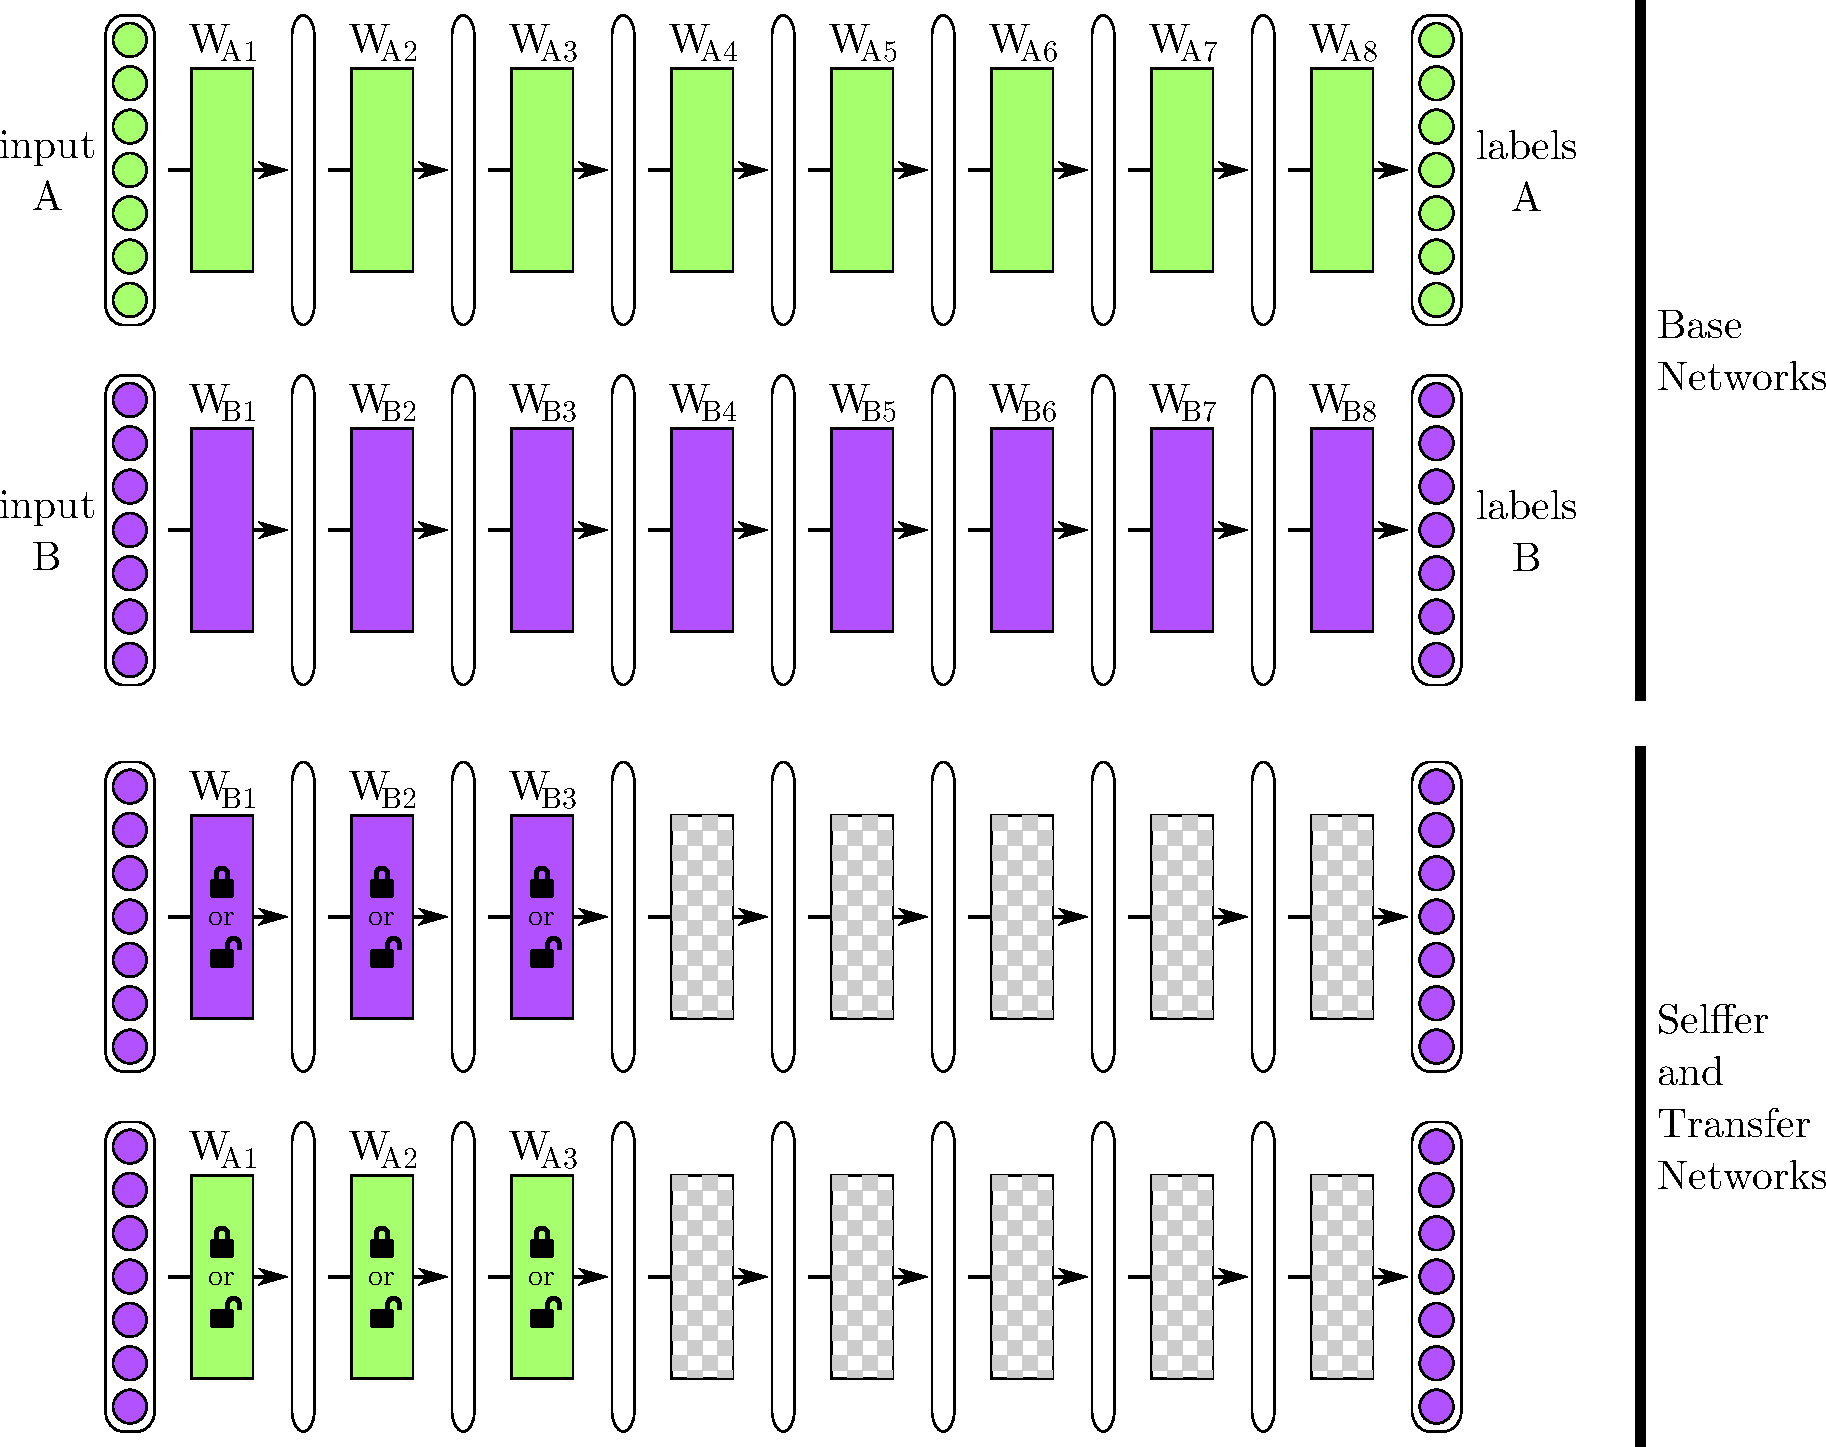
\includegraphics[width=1\linewidth]{drawings/transfer.pdf}
\end{center}
\caption{Overview of the experimental treatments and controls. \emph{Top two rows:} The baseline control involves training a Convolutional Network in the normal way \citep{Krizhevsky-2012}. Training occurs on only half the dataset (e.g. dataset A) for consistency with the experimental treatments. The baseline control is repeated for each half of the dataset (A and B). The labeled rectangles (e.g. $W_{A1}$) represent the weight vector for that layer. That the rectangle is colored indicates that the weight layer has been trained on the dataset of that color (e.g. dataset A). The vertical, ellipsoidal bars represent neural activations that occur when the network is activated. \emph{Third row:} In this control, the weights (filters) of all layers are initialized randomly (checkered pattern). The weights of the first $N$ layers of the network are locked, meaning they do not change during training. The remaining layers are trained as normal on half the dataset. A replicate (not pictured) is performed on the other half of the dataset. \emph{Fourth row:} The ``selfer network'' control. In this control the first $N$ weight layers of the network are copied from a base network (e.g. one trained on dataset B) and then the entire network is trained on that same dataset (in this example, dataset B). These layers are either locked during training (in the ``locked selfer treatments'') or allowed to train as usual (in the ``released selfer treatments''. The weights of layers after the first $N$ layers are initialized randomly and then allowed to train as usual. This treatment tests whether filters at different layers need to co-adapt during training, or if they can be trained asynchronously. \emph{Fifth row:} The ``transfer network'' experimental treatment. Same as the selfer network treatment, except that the first $N$ layers are copied from one half of the dataset (e.g. B) and then the entire network is trained on the \emph{other} half of the dataset (e.g. dataset A). This treatment tests transfer learning.}
\label{fig:transfer}
\end{figure}


The results for the random \dA/\dB splits are shown in Section~\ref{sec:experiments_ab}. Before proceeding, we note an important point about the random splits chosen in this way. ImageNet contains 1000 classes, some of which occur in clusters of related classes. For example, there happen to be many types of certain animals included in the dataset, particularly dogs and cats, like these 13 classes from the biological family \emph{Felidae}:

{
\small
\begin{verbatim}
   ID        Description
   n02123045 tabby, tabby cat
   n02123159 tiger cat
   n02123394 Persian cat
   n02123597 Siamese cat, Siamese
   n02124075 Egyptian cat
   n02125311 cougar, puma, catamount, mountain lion, Felis concolor
   n02127052 lynx, catamount
   n02128385 leopard, Panthera pardus
   n02128757 snow leopard, ounce, Panthera uncia
   n02128925 jaguar, panther, Panthera onca, Felis onca
   n02129165 lion, king of beasts, Panthera leo
   n02129604 tiger, Panthera tigris
   n02130308 cheetah, chetah, Acinonyx jubatus
\end{verbatim}
}

Because each randomly chosen \dA/\dB half will probably contain 6 or 7 of these felids, each half will have detectors trained on all levels to classify some types of felids. When generalizing to the other half, we would expect that the new high-level felid detectors trained on top of fixed old low-level felid detectors would work well.

For comparison, we've also created a special split of the dataset into two halves that are as far apart from each other as possible: one category containing only \emph{natural} classes and another containing \emph{man-made} objects. This split is not quite even --- there are 449 classes in the natural group and 551 in the man-made group. In Section~\ref{sec:experiments_random_nm} we show (a) how features transfer more poorly (so we say the are more specific) across this larger generalization gap and (b) how the generality of subsequent layers falls of smoothly.

\edit{mention faster training here}



\section{Details of Experimental Setup}

Since \cite{Krizhevsky-2012} won the ImageNet 2012 competition, there has naturally been much interest and work toward tweaking hyperparameters of large convolutional models. For example, \cite{Zeiler+et+al-arxiv2013b} found that it is better to decrease the first layer filters sizes from $11\times 11$ to $7\times 7$ and to use a smaller stride of $2$ instead of $4$. When beginning this study we faced the decision of exactly which convolutional architecture to use for our experiments. We decided to use the original architecture from \cite{Krizhevsky-2012} not to maximize absolute performance, but to study transfer results on what is probably the most popular single architecture, so that our results will be comparable, extensible, and useful to the largest number of other researchers. We actually expect none of the qualitative results presented here to depend at all on small architecture tweaks.

To this end, we used the hyperparameters provided in the reference implementation of  \cite{Krizhevsky-2012} with Caffe, a library for training convolutional models on a GPU \citep{donahue+jia-2013-arxiv}. We followed \citet{donahue+jia-2013-arxiv} in making a few minor departures from \cite{Krizhevsky-2012}: we skip the data augmentation trick of adding random multiples of principle components of pixel RGB values, which produced only a $1\%$ improvement in the original paper, and we warped images to $256\times 256$ instead of scaling to keep the aspect ratio and then cropping. In another difference, we placed the Local Response Normalization layers just \emph{after} the pooling layers, instead of before them. As in previous studies, we use Dropout \citep{Hinton-et-al-arxiv2012} on fully connected layers except for the softmax output layer.


For clarity of presentation, we list all hyperparameter selections in two tables: layer sizes and locations in Table~\ref{tab:network_architecture} and weight initialization and learning rate details in Table~\ref{tab:learning_hyperparams}. In the first table, a feedforward pass proceeds from top to bottom, left to right. Because code is often more clear than text, we've also made all code and parameter files necessary to reproduce these experiments available on \url{http://github.com/...removed_for_review...}.


\begin{table}[t]
\caption{Convolutional Network architecture sizes and hyperparameters. Conv stands for Convolutional layers. FC stands for fully-connected layers. R/S indicates that the layer consists of rectilinear or sigmoidal neurons. Neurons in dropout layers fail to fire with 50\% probability \todo{accurate?} \citep{Hinton-et-al-arxiv2012}\todo{Do we need to explain what groups means? Stride?} LRN stands for local response normalization \citep{Krizhevsky-2012}.}
\label{tab:network_architecture}
\begin{center}
\begin{tabular}{|r|l|l|l|l|l|l|l|l|l|}
\hline
       &      & filter & number  &        &        &     &         & Maxpool        & LRN (size,        \\
name   & pad  & size   & outputs & groups & stride & R/S & Dropout & (width,stride) & $\alpha$,$\beta$) \\
\hline
conv1  &      & 11x11  & 96      & 1      & 4      & R   &         & 3, 2           & 5,0.0001,0.75     \\
conv2  & 2    & 5x5    & 256     & 2      & 1      & R   &         & 3, 2           & 5,0.0001,0.75     \\
conv3  & 1    & 3x3    & 384     & 1      & 1      & R   &         &                &                   \\
conv4  & 1    & 3x3    & 384     & 2      & 1      & R   &         &                &                   \\
conv5  & 1    & 3x3    & 256     & 2      & 1      & R   &         & 3, 2           &                   \\
fc6    &      &        & 4096    & 1      &        & R   & *       &                &                   \\
fc7    &      &        & 4096    & 1      &        & R   & *       &                &                   \\
fc8    &      &        & 1000    & 1      &        & S   &         &                &                   \\
\hline
\end{tabular}
\end{center}
\end{table}




\begin{table}[t]
\caption{Parameter initializations and learning rates. \todo{JY: I expanded the table headings (we have the space). Please check that I did so accurately. I had to guess on most.}}
\label{tab:learning_hyperparams}
\begin{center}
\begin{tabular}{|r|l|l|l|l|l|l|}
\hline
       & \multicolumn{3}{c|}{\bf Weight}     &  \multicolumn{3}{c|}{\bf Bias}       \\
\cline{2-7}
       & Gaussian Std. Dev.   & Local Response-multiplier & decay &  const  & Local Response  & decay \\
\hline
conv1  & .01    & 1       & y     &  0      & 2   & n     \\
conv2  & .01    & 1       & y     &  1      & 2   & n     \\
conv3  & .01    & 1       & y     &  0      & 2   & n     \\
conv4  & .01    & 1       & y     &  1      & 2   & n     \\
conv5  & .01    & 1       & y     &  1      & 2   & n     \\
fc6    & .005   & 1       & y     &  1      & 2   & n     \\
fc7    & .005   & 1       & y     &  1      & 2   & n     \\
fc8    & .01    & 1       & y     &  0      & 2   & n     \\ 
\hline
\end{tabular}
\end{center}
\end{table}

We used stochastic gradient descent (SGD) with momentum. Each iteration of SGD used a batch size of 256, momentum 0.9, and multiplicative weight decay (for those weights with weight decay enabled) of 0.0005 per iteration.

For the bulk of the experiments in this paper, the master learning rate was started at 0.01, annealed over the course of training by dropping it by a factor of 10 every 100,000 iterations, and learning was stopped after 450,000 iterations. All training was done on NVidia K20 GPUs. Each iteration took about 1.7 seconds, meaning that the whole training procedure for a single network takes 9.5 days.

Because occupying a whole GPU for this long was cumbersome, we also devised a set of hyperparameters to allow faster learning by boosting the learning rate by 25\% to 0.0125, annealing by a factor of 10 after only 64,000 iterations, and stopping after 200,000 iterations. These selections were made after looking at the learning curves for the base case and estimating at which points in each region of constant learning rate the learning had plateaued and thus annealing could take place.
\edit{A typical learning curve is shown in Figure~\ref{typical_learning}.}


\editbox{
Figure {typical\_learning}
(( make this figure, if important, once reduced-1300-2 run is done ))
}

Our base model attains a final top-1 error on the validation set of 42.5\%, about the same as the 42.9\% reported by \cite{donahue+jia-2013-arxiv} and 1.8\% worse than \cite{Krizhevsky-2012}, the latter difference probably due to the few minor training differences. We checked these values only to demonstrate that the network was converging reasonably. As our goal is not to improve the state of the art, but to investigate properties of transfer, we were content with this level of performance.





%%%%%%%%%%%%%%%%%%%%%%%%%%%%%%%
%%%%%%%%%%%%%%%%%%%%%%%%%%%%%%%
%%%%%%%%%%%%%%%%%%%%%%%%%%%%%%%

\section{Transfer Results and Discussion}
\label{sec:experiments}


As mentioned earlier, we did two sets of experiments. The main experiment using random random \dA/\dB splits is discussed in Section~\ref{sec:experiments_ab}, and the two comparison cases using random filters and the Natural/Man-made split is presented in Section~\ref{sec:experiments_random_nm}.




\subsection{Random \dA/\dB splits}
\label{sec:experiments_ab}


\begin{figure}[htpb]
\begin{center}
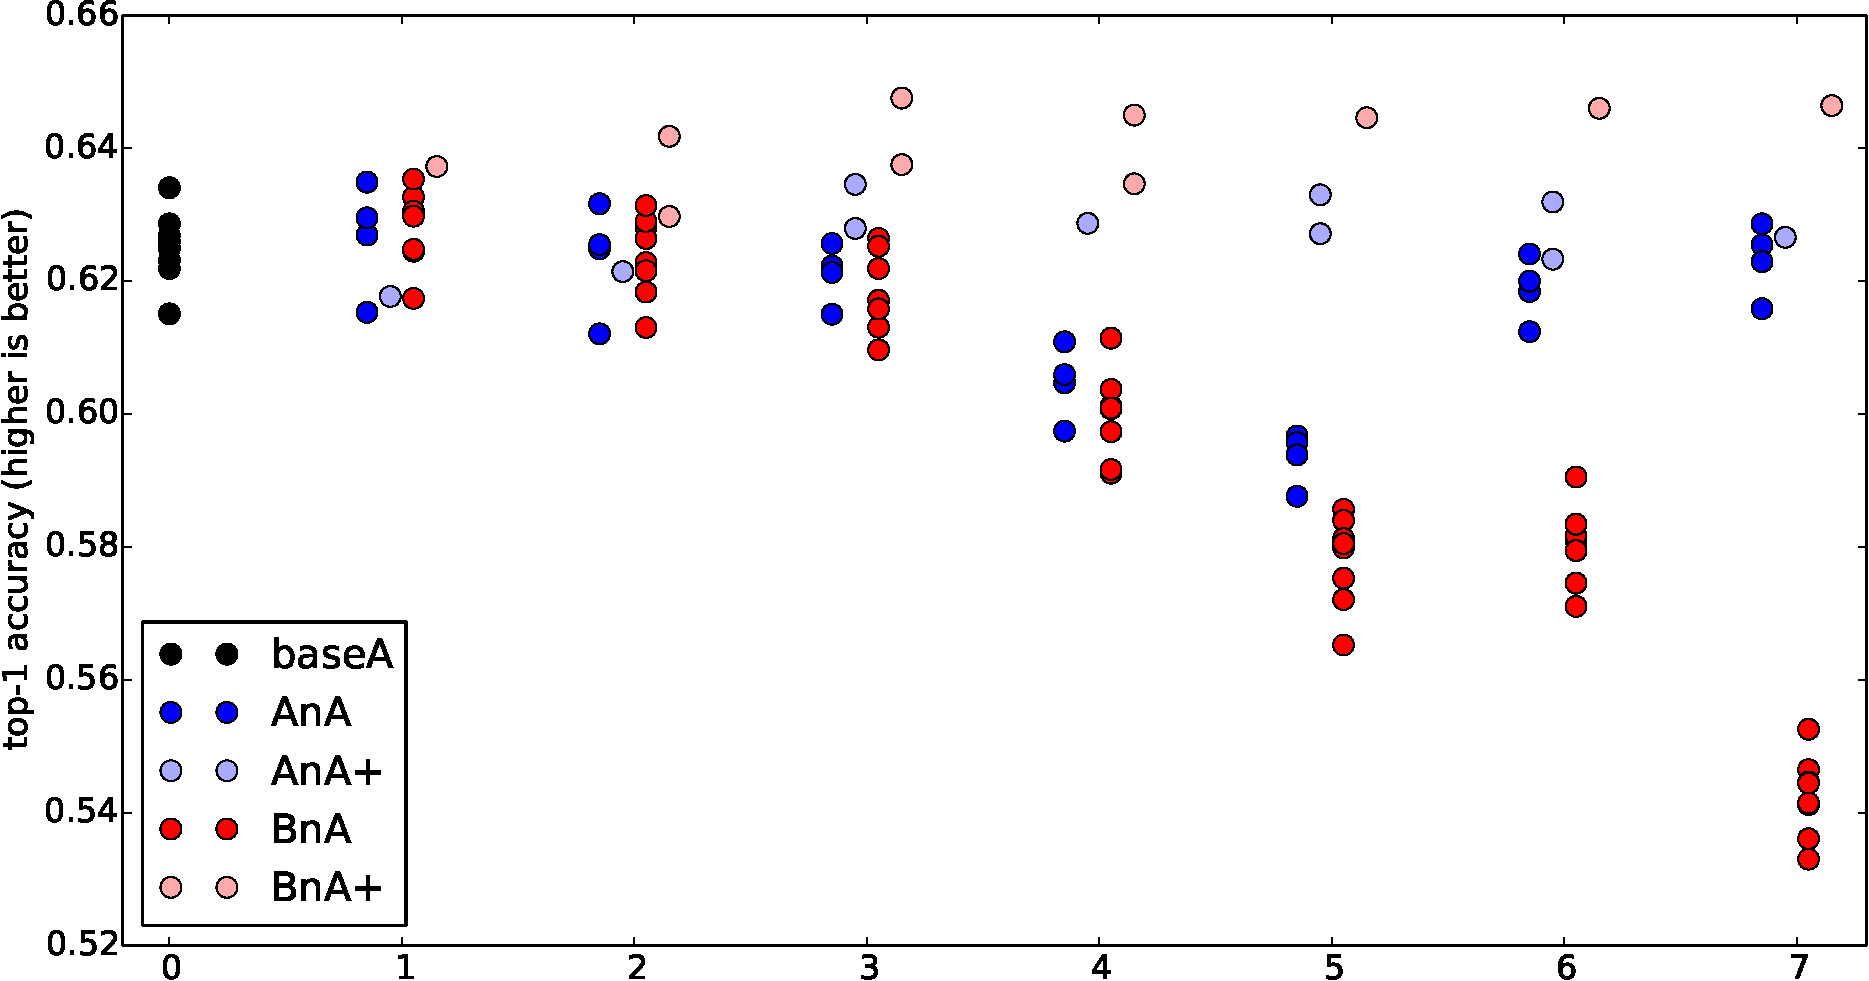
\includegraphics[width=1\linewidth]{plots/result_transfer_crop.pdf}
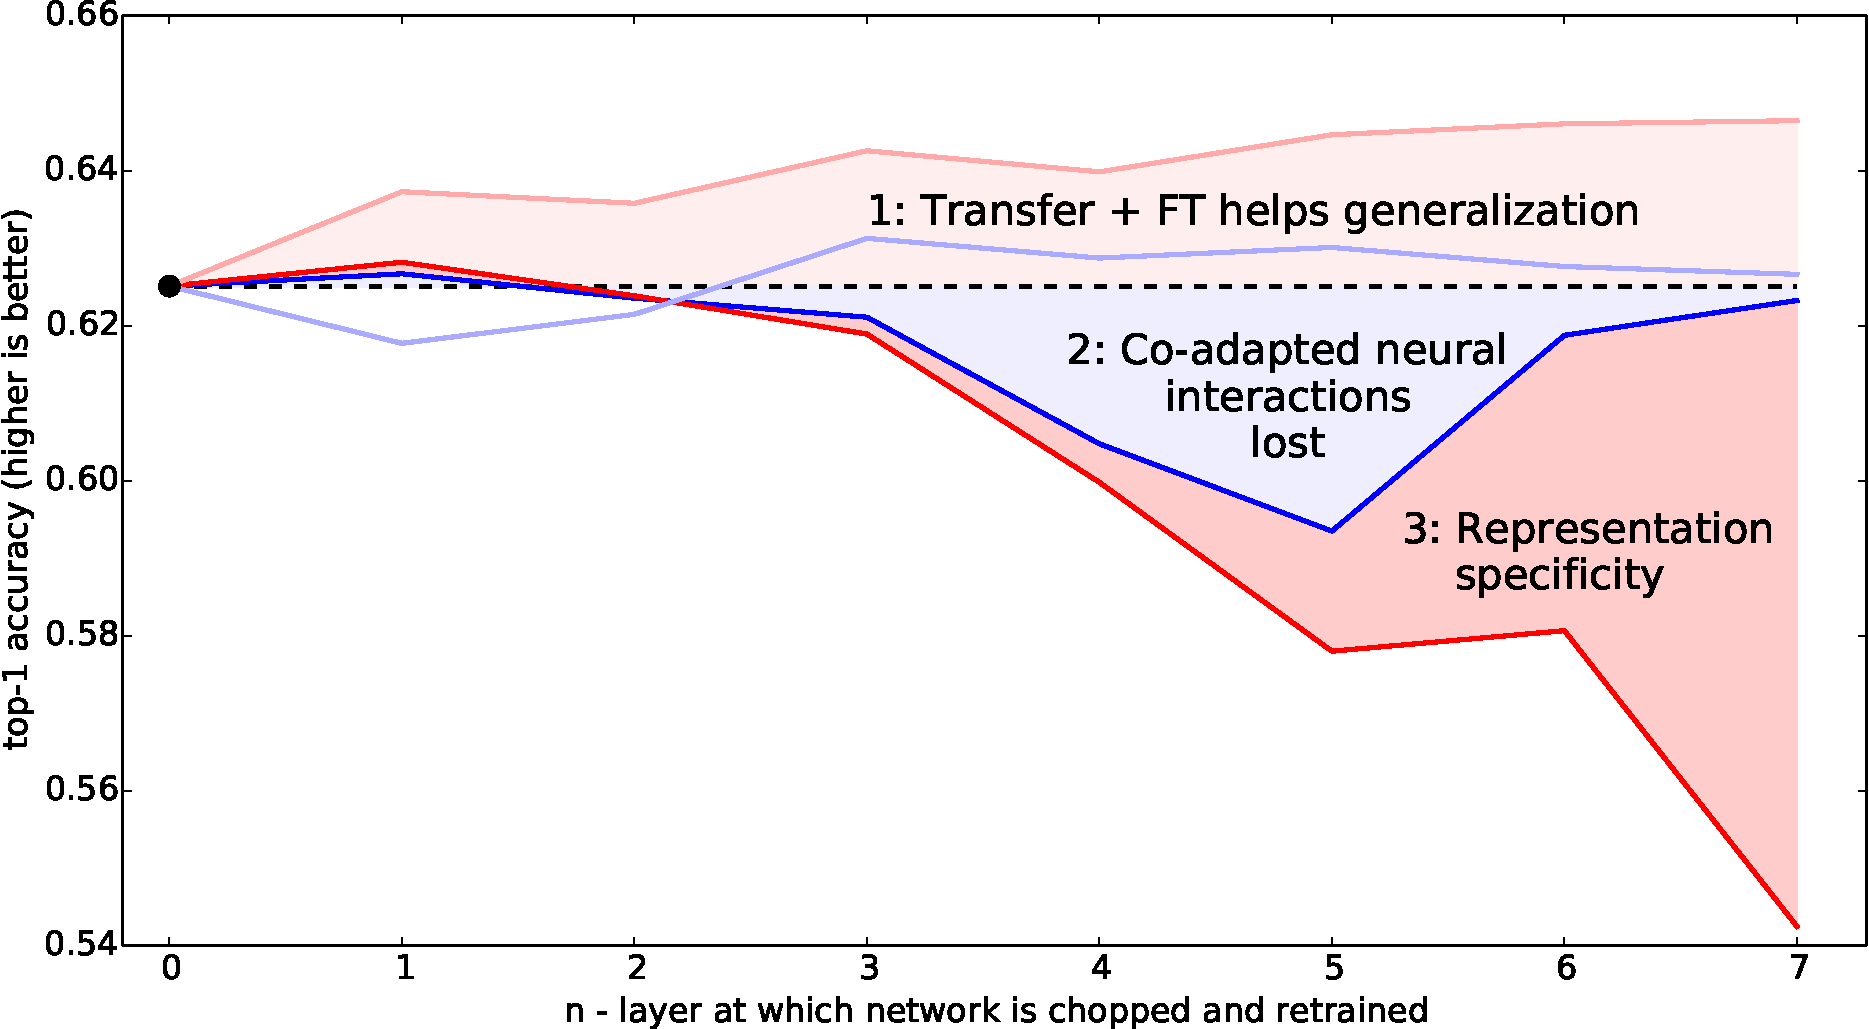
\includegraphics[width=1\linewidth]{plots/result_transfer_lines_crop.pdf}
\end{center}
\caption{Accuracy of each treatment and control. \emph{Top panel:} Raw data. \emph{Bottom panel}: Lines connect the medians of each treatment. Shaded areas and text highlight key takeaway messages. \todo{This is the min. required if we explain the figure in the main text.}
}
\label{fig:results}
\end{figure}

The results of all transfer learning experiments are shown in condensed form in Figure~\ref{fig:results}. Each dot in the figure represents the average accuracy over the validation set for an entire trained network. The black dots above $n=0$ represent the accuracy of \net{baseA} or \net{baseB}. There are eight points, because we made four separate random \net{A}/\net{B} splits. Each dark blue dot represents an \net{AnA} network\footnote{Actually these dots represent \net{AnA} nets or \net{BnB} nets, the statistics of which are equivalent, because in both cases the net is trained on the same random 500 classes. To simplify notation, we'll just calling these \net{AnA} networks. Similarly, we've aggregated the \net{BnA} and \net{AnB} networks and just call them \net{BnA}}, that is, a network that was trained on dataset \dA, chopped off at layer $n$, and then whose upper layers were reinitialized and retrained toward dataset \dA while the lower layers remained frozen. The light blue points represent \net{AnA^+} networks, the same as \net{AnA} but where the lower layers were fine-tuned as well. Each dark red dot represents a \net{BnA} network, one whose first $n$ layers are copied from \net{baseB} and frozen, and then whose upper layers were randomly initialized and trained toward dataset \dA. The light red points represent \net{BnA^+} networks where all layers were fine-tuned.

In the top subplot plot we've shifted each type of point slightly to the left or write simply for visual clarity; if not for this shift they would all be shown directly above $n=1$, $n=2$, etc. and would overlap. In the bottom subplot we've average the results at each layer to show more clearly the overall trend and to highlight the three important effects.

It turns out we can conclude quite a lot from these results! In each of the following interpretations, we compare the performance to the base case (black dots).

\begin{enumerate}

\item The black \net{baseA} points show that the mean performance of a network simply trained to classify a random subset of 500 classes attains a top-1 accuracy of 0.625, or 37.5\% top-1 error. This is different than the 42.5\% top-1 error attained on the 1000 class network for a combination of two reasons: it is pushed higher because the network is trained only on half of the data, which could lead to more overfit, and it is pushed lower because there are only 500 classes, so there are only half as many ways to make mistakes. It is this latter effect that dominates, leading to lower error overall.

\item The dark blue \net{AnA} points show a curious behavior. We can see at layer one that the performance is the same (as the \net{baseA} points), which was expected. If we learn eight layers of features, save the first layer of learned Gabor features, and reinitialize the whole network and retrain it toward the same task, we'd expect to do just as well. This is also true for layer 2. Layers 3, 4, 5, and 6, particularly 4 and 5, behave somewhat differently. When we keep the first, say, 5 layers and retrain layers 6-8, performance suffers. This is evidence that the original network contained \emph{co-adapted features} on successive layers, that is features that interact with each other in a complex way such that this co-adaptation \emph{could not be relearned} by the upper layers. In other words, gradient descent was able to find a good solution the first time, but this was only possible because the layers were jointly trained. As we continue to the right, we see that layer 6 is nearly back to the base level of performance, as is layer 7. As we get closer and closer to the final 500-way softmax output layer (8), there is less to relearn, and apparently relearning these one or two layers is simple enough for gradient descent to find a good solution. Alternately, we may say that there is less co-adaptation of features between layers 6 and 7 or between 7 and 8.

We are not sure whether or not this effect has been previously observed in the literature. Certainly one would suspect that optimization difficulties might occur, but we do not believe it has been previously shown that such difficulties are worse in the middle of a network than near the bottom or top.

\item The light blue \net{AnA^+} points show that, as expected, when we allow the copied lower layer features to learn as well, we're able to find a solution just as good as the original solution. The whole network is trained, just initialized from a partial previous solution instead of completely randomly, which neither helps nor hurts performance.

\item The dark red \net{BnA} points show the effect we set out to measure in the first place: the transferability of features from one network to another at each layer. Layers one and two transfer almost perfectly from \net{B} to  \net{A}, giving evidence that at least for our two tasks, not only are the Gabor features general, but the second layer features are as well. Layer three shows a slight drop, and layers 4-7 show a more significant drop in performance. Thanks to the \net{ANA} points, we can tell that this drop is from a combination of two separate effects: the drop from lost co-adaptation \emph{and} the drop from features which are less and less general. On layers 3, 4, and 5, the first effect dominates, whereas on layers 6 and 7 the first effect diminishes and the specificity of representation dominates the drop in performance.

Although examples of successful feature transfer have been reported elsewhere in the literature, to our knowledge these results have been limited to noticing that transfer from a given layer is much better than chance, e.g. noticing that the \net{BnA} points are much better than chance level performance (.002 for 500 classes). We believe this is the first time that the extent to which transfer is successful has been carefully quantified layer by layer and that the two separate effects have been decoupled, showing that each effect dominates in part of the regime.

\item The light red \net{BnA^+} points show perhaps the most surprising effect: that transferred features followed by fine-tuning result in networks that generalize better than those trained directly on the target dataset. We suspected that this effect might be simply due to longer total training time (450k base + 450k fine-tuned for \net{BnA^+} vs. 450k for \net{baseA}), but this cannot be the case, because the \net{AnA^+} networks are also trained for the same longer length of time and do not exhibit this boost in performance.

Thus, the most likely explanation is that even after 450k iterations of fine tuning (beginning with completely random top layers), the effects of having seen the alternate dataset still linger, boosting generalization performance. We found surprising the fact that this effect can linger through so much retraining. Further, this lingering boon to generalization seems not to depend very much on how much of the first network we keep to initialize the second network: keeping anywhere from one to seven layers produces improved performance, with slightly better performance as we keep more layers. The average boost across layers 1 to 7 is 1.6\% over the base case, and the average if we keep at least five layers is 2.1\%.\footnote{It is somewhat strange for us to aggregate the performance over several layers. Indeed, we'd prefer to average many runs at the same layer, but each point is rather computationally expensive to obtain so we have very few as of the time of this submission. However, we think some aggregation is informative, because the performance at each layer is based on completely different random draws of initialization weights. Thus, the fact that layers 5, 6, and 7 result in almost identical performance across random draws is at least somewhat indicative that multiple runs at a given layer would result in similar performance.} The degree of performance boost is shown in Table~\ref{tab:boost}.

\end{enumerate}

% Computed like this (set LAYER = {1,3,5})
%
% LAYER = 1
% nested = [list(mb_selffer_ft[ii]['valid_top1_acc']) for ii in range(LAYER,8)]
% case_selffer = array([item for sublist in nested for item in sublist])
% 
% nested = [list(mb_transfer_ft[ii]['valid_top1_acc']) for ii in range(LAYER,8)]
% case_transfer = array([item for sublist in nested for item in sublist])
% 
% print 'transfer - selffer', case_transfer.mean() - case_selffer.mean()
% print 'transfer - base',    case_transfer.mean() - case_base.mean()
% 
% #print stats.ttest_rel(case_base, case_selffer)
% print 'base    vs selffer ', stats.ttest_ind(case_base, case_selffer)
% #print stats.ttest_rel(case_base, case_transfer)
% print 'base    vs transfer', stats.ttest_ind(case_base, case_transfer)
% print 'selffer vs transfer', stats.ttest_ind(case_selffer, case_transfer)


\begin{table}[t]
\caption{Performance accuracy boost of transfer + fine-tuning \net{BnA^+} over controls. All differences are significant at the $p < .001$ level.}
\label{tab:boost}
\begin{center}
\begin{tabular}{|c|c|c|}
\hline
           & mean boost  & mean boost \\
layers     & over        & over \\
aggregated & \net{baseA} & selffer \net{AnA^+} \\
\hline
1-7        & 1.6\%       & 1.4\% \\
3-7        & 1.8\%       & 1.4\% \\
5-7        & 2.1\%       & 1.7\% \\
\hline
\end{tabular}
\end{center}
\end{table}



\subsection{Random filters and Natural/Man-made split}
\label{sec:experiments_random_nm}

In this section we compare the transfer performance of our random \dA/\dB splits to a control --- completely random filters --- and to our manually created 449 vs. 551 class natural/man-made split.

We make the first comparison because \cite{Jarrett-ICCV2009} showed, --- quite strikingly --- that the combination of random convolutional features, rectification, pooling, and local normalization can work almost as well as learned features. They showed this on relatively small networks of two or three learned layers and on a smaller dataset; and it is natural to ask whether or not the nearly optimal performance of random filters carries over to a deeper network trained on a larger dataset.

We make the second comparison to see how features transfer between two tasks that are as far apart as possible using the ImageNet dataset. Many are using and will use features trained from ImageNet for completely new tasks, and this second control gives some idea of how well features from various layers will transfer.

\begin{figure}
\begin{center}
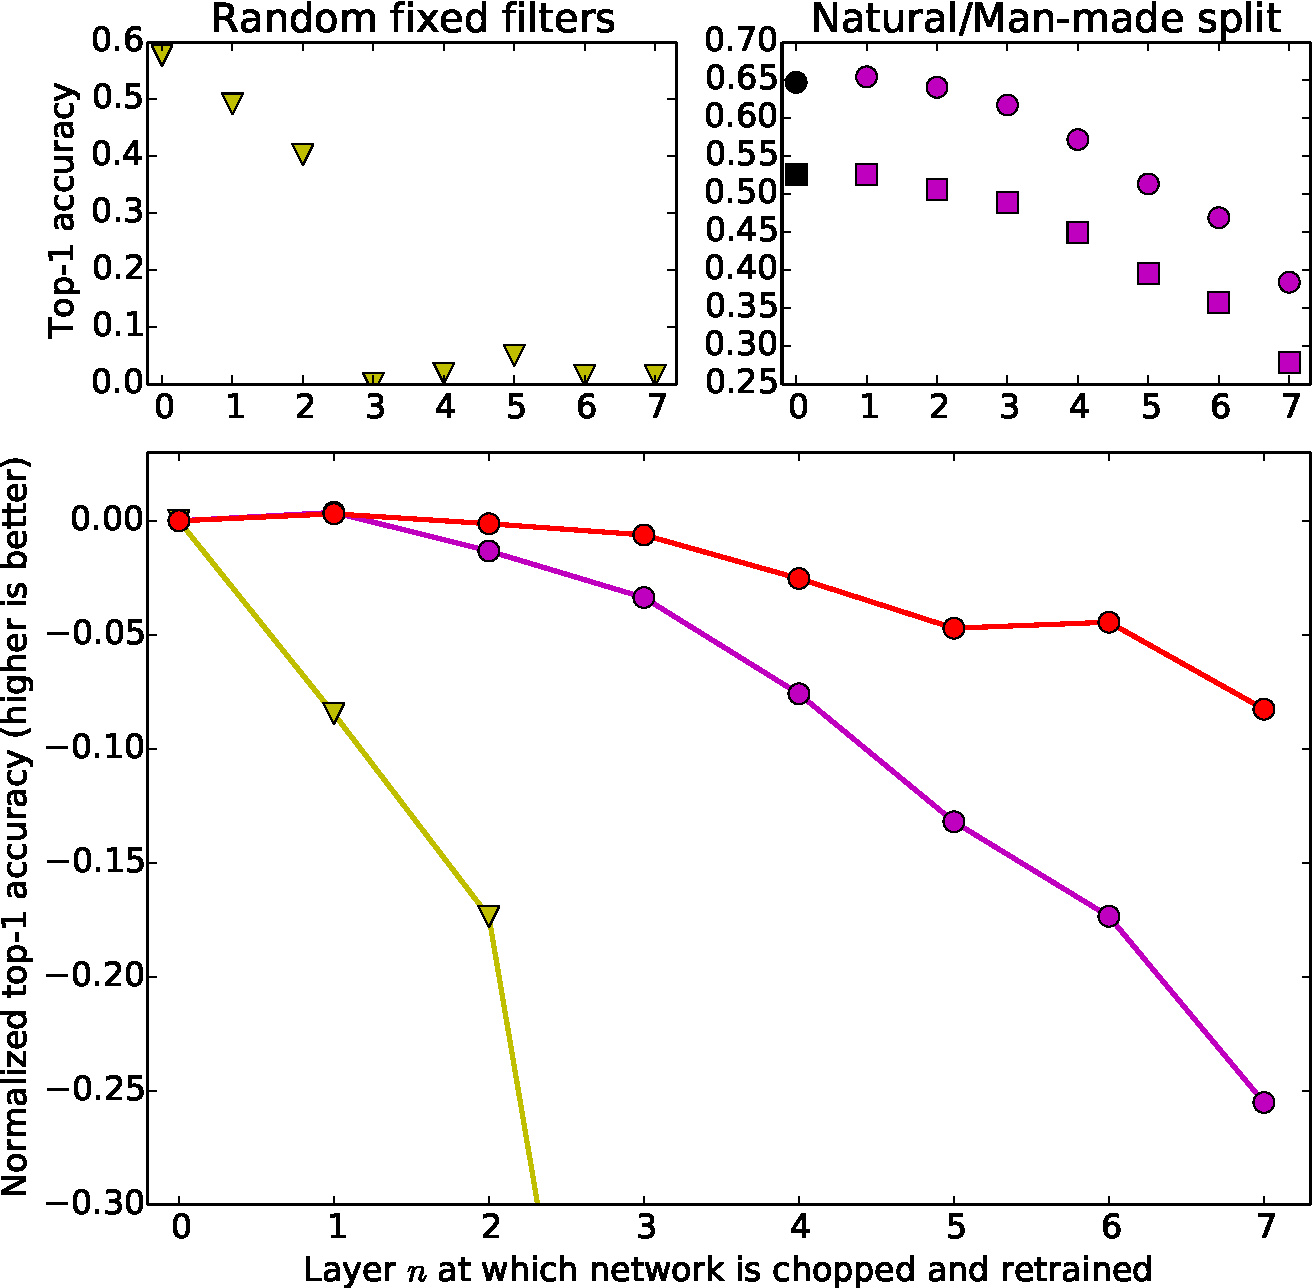
\includegraphics[width=1\linewidth]{plots/result_random_nm_combined_crop.pdf}
\end{center}
\caption{\edit{Caption here...}}
\label{fig:random_and_nm}
\end{figure}

Figure~\ref{fig:random_and_nm} shows the results of these two additional experiments. The upper-left subplot shows the accuracy obtained when using random filters for the first $n$ layers, for various choices of $n$. Performance falls off fairly quickly in layers 1 and 2, which suggests that getting random features to work in general convnets may not be as straightforward as it was for the smaller network size and smaller dataset used by \cite{Jarrett-ICCV2009}. However, the comparison is a bit tricky, because whereas we use max pooling and local normalization on layers 1 and 2 just as they did, we use a different nonlinearity: $\mathrm{relu}(x)$ instead of $\mathrm{abs}(\mathrm{tanh}(x))$. The difference in performance could be due to a few factors: slightly different nonlinearity, the dataset itself, sizes of critical pieces of the network, etc. Their experiment only considered two layers of random features. In our case and with our chosen hyperparameters, we see that by the third layer of random features, accuracy has dropped nearly to the chance level. Of course, this represents only one datapoint, and it may well be possible to tweak layer sizes and random initialization magnitudes to enable much better performance.

The upper-right subplot of Figure~\ref{fig:random_and_nm} shows the accuracy of the \net{baseA} (black circle), \net{baseB} (black square), \net{BnA} (magenta circles), and \net{AnB} (magenta squares) networks. The \net{baseA} and \net{BnA} networks are both eventually trained toward \dA, which is the natural half of the split and has higher average performance. This may be due to having only 449 classes instead of 551, or simply being an easier task, or both.

Finally, in the bottom plot of Figure~\ref{fig:random_and_nm} we normalize these several experiments by subtracting the performance of their individual base cases (which vary from each other for reasons mentioned above). We then plot the relative drop in performance as we use more random layers or pull more layers from a network trained on another dataset. This comparison makes two things apparent: first, that the transferability gap between two randomly selected \dA and \dB halves grows more slowly with increasing layer than does the transferability gap between two less related halves, and second, that for this network architecture, transferring even from a distant task is better than just using random filters. This latter result may hold because the networks trained in \citep{Jarrett-ICCV2009} could have been well into the overfitting regime on a dataset as small as Caltech-101 \citep{Fei-Fei.2004}.



\section{Conclusions}



Practical conclusions

If you don't have a big second dataset:

Results 2 and 4 imply that those wishing to transfer features from one dataset to another face not only the problem of specificity, but....



If you do have a big second dataset:




A final thing to notice is that all layers are fairly general. Even the networks in column 7, in which only the final 500-way softmax layer is retrained to the new dataset, suffer only an 8\% accuracy drop in the A/B split case, but a much larger 25\% drop in the natural/manmade case. In the natural/man-made split case, the drop is fairly smooth through the network

